% Copyright 2007 by Till Tantau
%
% This file may be distributed and/or modified
%
% 1. under the LaTeX Project Public License and/or
% 2. under the GNU Public License.
%
% See the file doc/licenses/LICENSE for more details.



\documentclass{beamer}

%
% DO NOT USE THIS FILE AS A TEMPLATE FOR YOUR OWN TALKS�!!
%
% Use a file in the directory solutions instead.
% They are much better suited.
%


% Setup appearance:

\usetheme{Darmstadt}
\usefonttheme[onlylarge]{structurebold}
\setbeamerfont*{frametitle}{size=\normalsize,series=\bfseries}
\setbeamertemplate{navigation symbols}{}


% Standard packages

\usepackage[english]{babel}
\usepackage[latin1]{inputenc}
\usepackage{times}
\usepackage[T1]{fontenc}
\usepackage{wasysym}
\usepackage[normalem]{ulem}               % to striketrhourhg text
\newcommand\redout{\bgroup\markoverwith
{\textcolor{red}{\rule[0.5ex]{2pt}{0.8pt}}}\ULon}


% Setup TikZ

\usepackage{tikz}
\usetikzlibrary{arrows}
\tikzstyle{block}=[draw opacity=0.7,line width=1.4cm]


% Author, Title, etc.

\title[]
{%
Computing Minimal Unsatisfiable Subsets of Constraints%
}

\author[Robbani]
{
	Author: Shahriar Robbani
	\\ Supervision: Erika \'{A}brah\'{a}m
}

\institute[]
{
	Theory of Hybrid Systems - Informatik 2 - RWTH-Aachen
}

\date[WABI 2006]
{Seminar Winter-16/17}



% The main document

\begin{document}

\begin{frame}
	\titlepage
\end{frame}

\begin{frame}{Outline}
	\tableofcontents
\end{frame}

\section{Fundamentals}
\begin{frame}{Fundamentals}
	\begin{itemize}
		\item \textbf{Propositional Logic Formula:}
		A well-formed propositional logic has following grammar:
		$$\varphi\hspace{3mm} :=\hspace{3mm} a\hspace{3mm} |\hspace{3mm} (\neg \varphi)\hspace{3mm} |\hspace{3mm} (\varphi \wedge \varphi)$$
		\item \textbf{Literals:}
		A literal is a positive or negative instance of Boolean variable. For example, $x$ or $\neg x$.
		\item \textbf{Clause:} It is a disjunction of literals. For example, $C = (a \vee \neg b \vee c)$.
		\item \textbf{Conjunctive Normal Form (CNF):} A CNF formula $\varphi$ is defined as follows:
		$$\varphi = \bigwedge\limits_{i=1\ldots n} C_{i}$$
		\item \textbf{Clause-Selector Variable:}  A clause-selector variable, $w_{i}$  is defined as:
		$$C^{\prime}_{i}=(\neg w_{i}\vee C_{i})$$
	\end{itemize}
\end{frame}


\begin{frame}{Minimal Unsatisfiable Subsets and Minimal Correction Subset}
	\begin{enumerate}[]
		\item <1-> \textbf{Minimal Unsatisfiable Subset (MUSs):} 
		\begin{table}[]
			\centering
			\begin{tabular}{|c|c|c|c|}
				\hline
				($x$) & ($\neg x$) & ($\neg x \vee y$) & ($\neg x \vee \neg y$) \\ \hline
				$\Square$   & $\Square$        &                &                     \\ \hline
				$\Square$   &         &        $\Square$        &                     \\ \hline
			\end{tabular}
		\end{table}
		\vspace*{\fill}
		\vspace*{\fill}
		\vspace*{\fill}
		\item <2-> \textbf{Minimal Unsatisfiable Subset (MUSs):} 
		\begin{table}[]
			\centering
			\begin{tabular}{|c|c|c|c|}
				\hline
				($x$) & ($\neg x$) & ($\neg x \vee y$) & ($\neg x \vee \neg y$) \\ \hline
				$\checkmark$   &            &                &                     \\ \hline
				&    $\checkmark$     &        $\checkmark$        &              \\ \hline
				&    $\checkmark$     &               &        $\checkmark$      \\ \hline
			\end{tabular}
		\end{table}
	\end{enumerate}
	\vspace*{\fill}
	\vspace*{\fill}
	\vspace*{\fill}
	\vspace*{\fill}
	\vspace*{\fill}
	$$\varphi=\underbrace{(x)}\limits_{C_{1}}\wedge\underbrace{(\neg x)}\limits_{C_2}\wedge\underbrace{(\neg x\vee y)}\limits_{C_{3}}\wedge\underbrace{(\neg x \vee \neg y)}\limits_{C_{4}}$$
\end{frame}


\begin{frame}{MUS $\setminus$ MCS Duality}
	\begin{itemize}
		\item \textbf{Hitting Sets:}
		\begin{enumerate}[]
			\item <1-> D = \{a, b, c, d\}
			\item <1-> $\Omega$ = \{({\only<2>{\color{red}}{\only<6>{\color{red}}{\only<7>{\color{cyan}}a}}},{\only<2>{\color{red}}{\only<3>{\color{green}}{\only<4>{\color{cyan}}{\only<8>{\color{green}}b}}}}),({\only<2>{\color{red}}{\only<3>{\color{green}}{\only<4>{\color{cyan}}{\only<8>{\color{green}}b}}}},{\only<3>{\color{green}}{\only<6>{\color{red}}c}},{\only<7>{\color{cyan}}d})\}
			\item <1-> H = \{({\only<2>{\color{red}}a},{\only<2>{\color{red}}b}), ({\only<3>{\color{green}}b},{\only<3>{\color{green}}c}), {\only<4>{\color{cyan}}b}, $ \ldots $\}
			\item <5-> MinH = \{({\only<6>{\color{red}}a},{\only<6>{\color{red}}c}), ({\only<7>{\color{cyan}}a},{\only<7>{\color{cyan}}d}), {\only<8>{\color{green}}b}\}
		\end{enumerate}
		\item <9-> The set of MUSs of a formula $\varphi$ is equal to the set of minimal hitting sets of the set of MCSs.
		\begin{enumerate}[]
			\item $ MCS_{1} = \{ {\only<10>{\color{red}}{\only<11>{\color{green}}C_{1}}} \} $
			\item $ MCS_{2} = \{ {\only<10>{\color{red}}C_{2}}, {\only<11>{\color{green}}C_{3}} \} $
			\item $ MCS_{3} = \{ {\only<10>{\color{red}}C_{2}}, {\only<11>{\color{green}}C_{4}} \} $
			\vspace*{\fill}
			\item $ MUS_{1} = \{{\only<10>{\color{red}}C_{1}}, {\only<10>{\color{red}}C_{2}}\} $
			\item $ MUS_{2} = \{ {\only<11>{\color{green}}C_{1}}, {\only<11>{\color{green}}C_{3}}, {\only<11>{\color{green}}C_{4}} \} $
		\end{enumerate}
	\end{itemize}
	\only<9->{$$\varphi=\underbrace{(x)}\limits_{C_{1}}\wedge\underbrace{(\neg x)}\limits_{C_2}\wedge\underbrace{(\neg x\vee y)}\limits_{C_{3}}\wedge\underbrace{(\neg x \vee \neg y)}\limits_{C_{4}}$$}
\end{frame}


\begin{frame}{MUS $\setminus$ MCS Duality (cnt...)}
	\begin{itemize}
		\item Additionally, each MCS is an minimal hitting set of the set of MUSs.
		\item So, minimal hitting sets of MUSs and MCSs provide a transformation from one collection to the other. This is the duality of MUS and MCS.
		\begin{figure}[htb]
			\begin{center}
				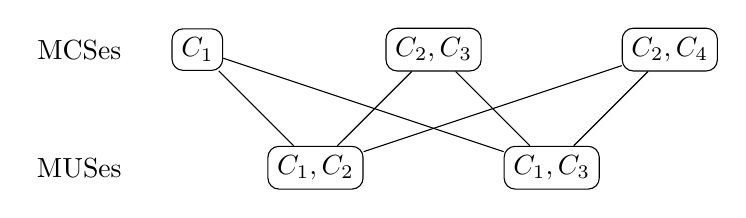
\begin{tikzpicture}[scale=1.5, 
				    state/.style={draw, rounded corners, fill=none,
				    			  text centered, text=black}]
	\node[] (u0) at (1, 2) {MCSes};
	\node[state] (u1) at (2, 2) {$C_{1}$};
	\node[state] (u2) at (4, 2) {$C_{2}, C_{3}$};
	\node[state] (u3) at (6, 2) {$C_{2}, C_{4}$};
	\node[state] (u4) at (3, 1) {$C_{1}, C_{2}$};
	\node[state] (u5) at (5, 1) {$C_{1}, C_{3}$};
	\node[] (u6) at (1, 1) {MUSes};
	
	\path[-] 	(u1)  edge   (u4);
	\path[-] 	(u1)  edge   (u5);
	\path[-] 	(u2)  edge   (u4);
	\path[-] 	(u2)  edge   (u5);
	\path[-] 	(u3)  edge   (u4);
	\path[-] 	(u3)  edge   (u5);

\end{tikzpicture}

			\end{center}
		\end{figure}
	\end{itemize}
	$$\varphi=\underbrace{(x)}\limits_{C_{1}}\wedge\underbrace{(\neg x)}\limits_{C_2}\wedge\underbrace{(\neg x\vee y)}\limits_{C_{3}}\wedge\underbrace{(\neg x \vee \neg y)}\limits_{C_{4}}$$
\end{frame}

\section{Algorithms for compution all MUSs}

\begin{frame}{Approach}
	\begin{enumerate}
		\item Computing all MCSs
		\item Computing Hitting Sets of MCSs
	\end{enumerate}
\end{frame}

\begin{frame}{Algorithm: Computing all MCSs}
	\begin{itemize}
		\item <1-> Augment CNF with clause selector variables
		$$\varphi=(x)\wedge(\neg x)\wedge(\neg x\vee y)\wedge(\neg x \vee \neg y)$$
		$$ \Downarrow $$
		$$\varphi^{\prime}=({\only{\color{red}}\neg w_{1}}\vee x)\wedge({\only{\color{red}}\neg w_{2}}\vee \neg x)\wedge({\only{\color{red}}\neg w_{3}}\vee \neg x\vee y)\wedge({\only{\color{red}}\neg w_{4}} \vee \neg x \vee \neg y)$$
		\item <2-> Find a solution to the augmented formula with the fewest $w$-variables assigned $\mathbf{false}$
				$$\varphi^{\prime}=(\neg {\only{\color{green}}\mathbf{false}} \vee x)\wedge(\neg w_{2}\vee \neg x)\wedge(\neg w_{3}\vee \neg x\vee y)\wedge(\neg w_{4}\vee \neg x \vee \neg y)$$
		\item <3-> Add blocking clauses to block old solutions
		$$\varphi^{\prime}=\varphi^{\prime} \wedge {\only{\color{cyan}} w_{1}}$$
		\item <4-> Find MCSs incrementally until all are found.
	\end{itemize}
\end{frame}

\begin{frame}{Example: Computing all MCSs}
			$$\varphi=\underbrace{(x)}\limits_{C_{1}}\wedge\underbrace{(\neg x)}\limits_{C_2}\wedge\underbrace{(\neg x\vee y)}\limits_{C_{3}}\wedge\underbrace{(\neg x \vee \neg y)}\limits_{C_{4}}$$
	\fbox{
		\begin{minipage}{6em}{Clauses}
			\fontsize{6}{9}\selectfont
			\begin{enumerate}
				\item <1> $x$
				\item <1> $\neg x$
				\item <1> $\neg x\vee y$
				\item <1> $\neg x \vee \neg y$
			\end{enumerate}
		\end{minipage}
	}
\end{frame}

\begin{frame}{Example: Computing all MCSs}
		$$\varphi=\underbrace{(x)}\limits_{C_{1}}\wedge\underbrace{(\neg x)}\limits_{C_2}\wedge\underbrace{(\neg x\vee y)}\limits_{C_{3}}\wedge\underbrace{(\neg x \vee \neg y)}\limits_{C_{4}}$$
		\fbox{
		\begin{minipage}{6em}{Clauses}
			\fontsize{6}{9}\selectfont
			\begin{enumerate}
				\item ${\only{\color{red}}\neg w_{1}}\vee x$
				\item ${\only{\color{red}}\neg w_{2}}\neg x$
				\item ${\only{\color{red}}\neg w_{3}}\neg x\vee y$
				\item ${\only{\color{red}}\neg w_{4}}\neg x \vee \neg y$
				\item <3-> ${\only{\color{green}}w_{1}}$
				\item <5-> ${\only{\color{green}}w_{2} \vee w_{3}}$
				\item <6-> ${\only{\color{green}}w_{2} \vee w_{4}}$
			\end{enumerate}
		\end{minipage}
	}
	\fbox{
	\begin{minipage}{10em}
	\fontsize{6}{9}\selectfont
		\begin{enumerate}
			\item <1-> Add clause-selector variables.
			\item <2-> Add AtMost constraint.
			\item <3-> First solution : w1 is $\mathbf{false}$. Add blocking clause and a MCS.
			\item <4-> No further solutions, increment AtMost.
			\item <5-> Second solution : w2 and w3 are $\mathbf{false}$. Add blocking clause and another MCSs.
			\item <6-> Third solution : w2 and w4 are $\mathbf{false}$. Add blocking clause and another MCSs.
			\item <7-> No further solutions, even without AtMost constraint.
		\end{enumerate}
	\end{minipage}
}
\only<3->{
\fbox{
	\begin{minipage}{7em}{MCSs}
		\fontsize{6}{9}\selectfont
		\begin{enumerate}
			\item <3-> ${\only{\color{cyan}}\{x\}}$
			\item <5-> ${\only{\color{cyan}}\{\neg x, \neg x\vee y\}}$
			\item <6-> ${\only{\color{cyan}}\{\neg x, \neg x\vee \neg y\}}$
		\end{enumerate}
	\end{minipage}
} }
\only<2-6>{$$AtMost(\{w_{1},w_{2},w_{3},w_{4}\}, \only<2-3>{1} \only<4-6>{2} )$$}
\end{frame}

\begin{frame}{Algorithm: Computing Hitting Sets of MCSs (For a Branch)}
	\begin{enumerate}[]
	\item $ MCS_{1} = \{x\}  $
	\item $ MCS_{2} = \{ \neg x , \neg x\vee y\} $
	\item $ MCS_{3} = \{ \neg x , \neg x\vee \neg y\} $
	\end{enumerate}
\begin{itemize}
	\item Select a clause to add to the growing set of MUS: $selClause= \neg x$, $MUS = \neg x$
	\item <2-> Select a MCS in which $selClause$ appears : $selMCS = MCS_{2}$, $newMCSs = MCSs$
\end{itemize}
	$$\varphi=\underbrace{(x)}\limits_{C_{1}}\wedge\underbrace{(\neg x)}\limits_{C_2}\wedge\underbrace{(\neg x\vee y)}\limits_{C_{3}}\wedge\underbrace{(\neg x \vee \neg y)}\limits_{C_{4}}$$
\end{frame}

\begin{frame}{Algorithm: Computing Hitting Sets of MCSs (For a Branch)}
	\begin{enumerate}[]
		\item $ MCS_{1} = \{x\}  $
		\item $ MCS_{2} = \{\neg x, $ \redout {$\neg x\vee y$}  $ \} $
		\item $ MCS_{3} = \{ \neg x, \neg x\vee \neg y\} $
	\end{enumerate}
	\begin{itemize}
		\item Select a clause to add to the growing set of MUS: $selClause= \neg x$, $MUS = \neg x$
		\item Select a MCS in which $selClause$ appears : $selMCS = MCS_{2}$, $newMCSs = MCSs$
		\item Remove any other clauses of $selMCS$ from each set of MCSs
	\end{itemize}
	$$\varphi=\underbrace{(x)}\limits_{C_{1}}\wedge\underbrace{(\neg x)}\limits_{C_2}\wedge\underbrace{(\neg x\vee y)}\limits_{C_{3}}\wedge\underbrace{(\neg x \vee \neg y)}\limits_{C_{4}}$$
\end{frame}


\begin{frame}{Algorithm: Computing Hitting Sets of MCSs (For a Branch)}
	\begin{enumerate}[]
		\item $ MCS_{1} = \{x\}  $
		\item \redout{$ MCS_{2} = \{\neg x\} $}
		\item \redout{$ MCS_{3} = \{ \neg x, \neg x\vee \neg y\} $}
	\end{enumerate}
	\begin{itemize}
		\item Select a clause to add to the growing set of MUS: $selClause= \neg x$, $MUS = \neg x$
		\item Select a MCS in which $selClause$ appears : $selMCS = MCS_{2}$, $newMCSs = MCSs$
		\item Remove any other clauses of $selMCS$ from each set of MCSs
		\item Remove MCSs from $newMCSs$ in which $selClause$ contains.
	\end{itemize}
	$$\varphi=\underbrace{(x)}\limits_{C_{1}}\wedge\underbrace{(\neg x)}\limits_{C_2}\wedge\underbrace{(\neg x\vee y)}\limits_{C_{3}}\wedge\underbrace{(\neg x \vee \neg y)}\limits_{C_{4}}$$
\end{frame}

\begin{frame}{Algorithm: Computing Hitting Sets of MCSs (For a Branch)}
	\begin{enumerate}[]
		\item $ MCS_{1} = \{x\}  $
	\end{enumerate}
	\begin{itemize}
		\item Select a clause to add to the growing set of MUS: $selClause= \neg x$, $MUS = \neg x$
		\item Select a MCS in which $selClause$ appears : $selMCS = MCS_{2}$, $newMCSs = MCSs$
		\item Remove any other clauses of $selMCS$ from each set of MCSs
		\item Remove MCSs from $newMCSs$ in which $selClause$ contains.
		\item Iterate until $newMCSs = \emptyset$, empty $ newMCSs $ is found by generating a MUS $\{x, \neg x\}$
	\end{itemize}
	$$\varphi=\underbrace{(x)}\limits_{C_{1}}\wedge\underbrace{(\neg x)}\limits_{C_2}\wedge\underbrace{(\neg x\vee y)}\limits_{C_{3}}\wedge\underbrace{(\neg x \vee \neg y)}\limits_{C_{4}}$$
\end{frame}


\begin{frame}{Example: Computing Hitting Sets of MCSs}
	\begin{figure}[htb] % where to insert the figure: h=here, t=top, b=bottom,
		% the order htb shows which position is preffered
		\begin{center}
			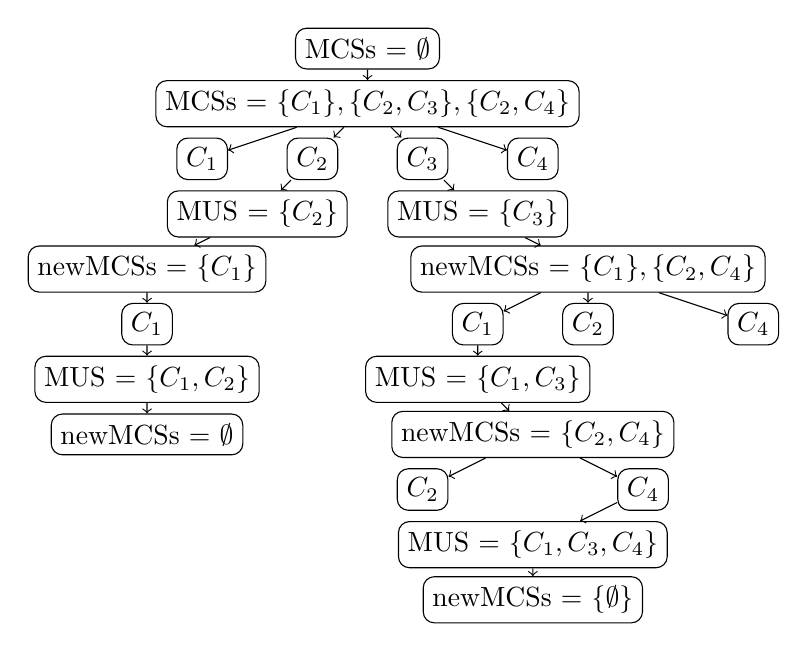
\begin{tikzpicture}[scale=0.7, 
			state/.style={draw, rounded corners, fill=none,
				text centered, text=black}]
			\node[state] (u0) at (5, 12) {MCSs = $\emptyset$};
			\node[state] (u1) at (5, 11) {MCSs = $\{C_{1}\}, \{C_{2},C_{3}\}, \{C_{2},C_{4}\}$};
			\node[state] (u2) at (2, 10) {$C_{1}$};
			\node[state] (u3) at (4, 10) {$C_{2}$};
			\node[state] (u4) at (6, 10) {$C_{3}$};
			\node[state] (u5) at (8, 10) {$C_{4}$};
			\node[state] (u6) at (3, 9) {MUS = $\{C_{2}\}$};
			\node[state] (u7) at (7, 9) {MUS = $\{C_{3}\}$};
			\node[state] (u8) at (1, 8) {newMCSs = $\{C_{1}\}$};
			\node[state] (u9) at (9, 8) {newMCSs = $\{C_{1}\}, \{C_{2}, C_{4}\}$};
			\node[state] (u10) at (1, 7) {$C_{1}$};
			\node[state] (u11) at (7, 7) {$C_{1}$};
			\node[state] (u12) at (9, 7) {$C_{2}$};
			\node[state] (u13) at (12, 7) {$C_{4}$};
			\node[state] (u14) at (1, 6) {MUS = $\{C_{1}, C_{2}\}$};
			\node[state] (u15) at (7, 6) {MUS = $\{C_{1}, C_{3}\}$};
			\node[state] (u16) at (1, 5) {newMCSs = $\emptyset$};
			\node[state] (u17) at (8, 5) {newMCSs = $\{C_{2}, C_{4}\}$};
			\node[state] (u18) at (6, 4) {$C_{2}$};
			\node[state] (u19) at (10, 4) {$C_{4}$};
			\node[state] (u20) at (8, 3) {MUS = $\{C_{1}, C_{3}, C_{4}\}$};
			\node[state] (u21) at (8, 2) {newMCSs = $\{\emptyset\}$};
			
			
			\path[->] 	(u0)  edge   (u1);
			\path[->] 	(u1)  edge   (u2);
			\path[->] 	(u1)  edge   (u3);
			\path[->] 	(u1)  edge   (u4);
			\path[->] 	(u1)  edge   (u5);
			\path[->] 	(u3)  edge   (u6);
			\path[->] 	(u4)  edge   (u7);
			\path[->] 	(u6)  edge   (u8);
			\path[->] 	(u7)  edge   (u9);
			\path[->] 	(u8)  edge   (u10);
			\path[->] 	(u9)  edge   (u11);
			\path[->] 	(u9)  edge   (u12);
			\path[->] 	(u9)  edge   (u13);
			\path[->] 	(u10)  edge   (u14);
			\path[->] 	(u11)  edge   (u15);
			\path[->] 	(u14)  edge   (u16);
			\path[->] 	(u15)  edge   (u17);
			\path[->] 	(u17)  edge   (u18);
			\path[->] 	(u17)  edge   (u19);
			\path[->] 	(u19)  edge   (u20);
			\path[->] 	(u20)  edge   (u21);
			\end{tikzpicture}
		\end{center}
	\end{figure}
\end{frame}

\begin{frame}%%     1
	\begin{center}
		\Huge Thank You! :)
	\end{center}
\end{frame}

\end{document}


